\subsection{Bubble \& eat - Cliente}
\begin{figure}[H]
	\centering
	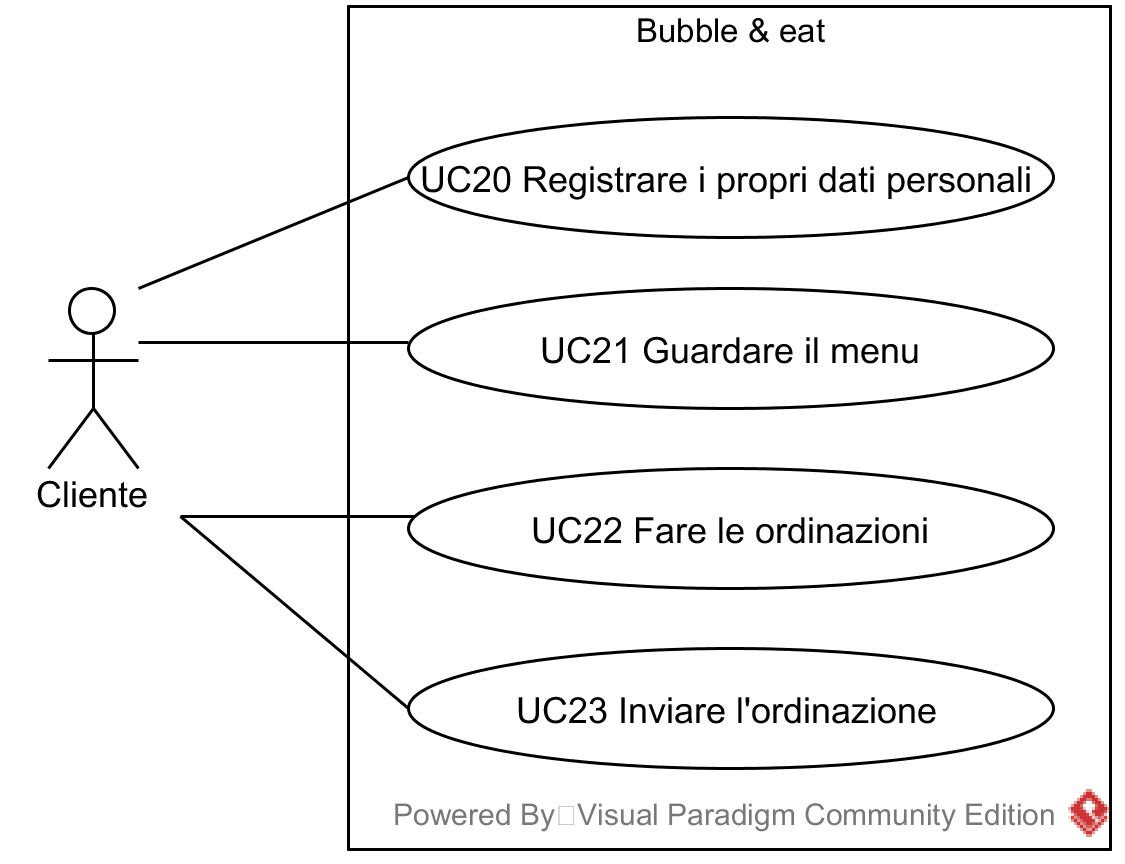
\includegraphics[width=15cm]{./Diagrammi_img/usecase/uc_bubble_client.png}
	\caption{Casi d'uso Bubble \& eat - Utente Cliente}
\end{figure}

\UC{Registrazione dei propri dati personali}{UC3.1}

\begin{figure}[H]
	\centering
	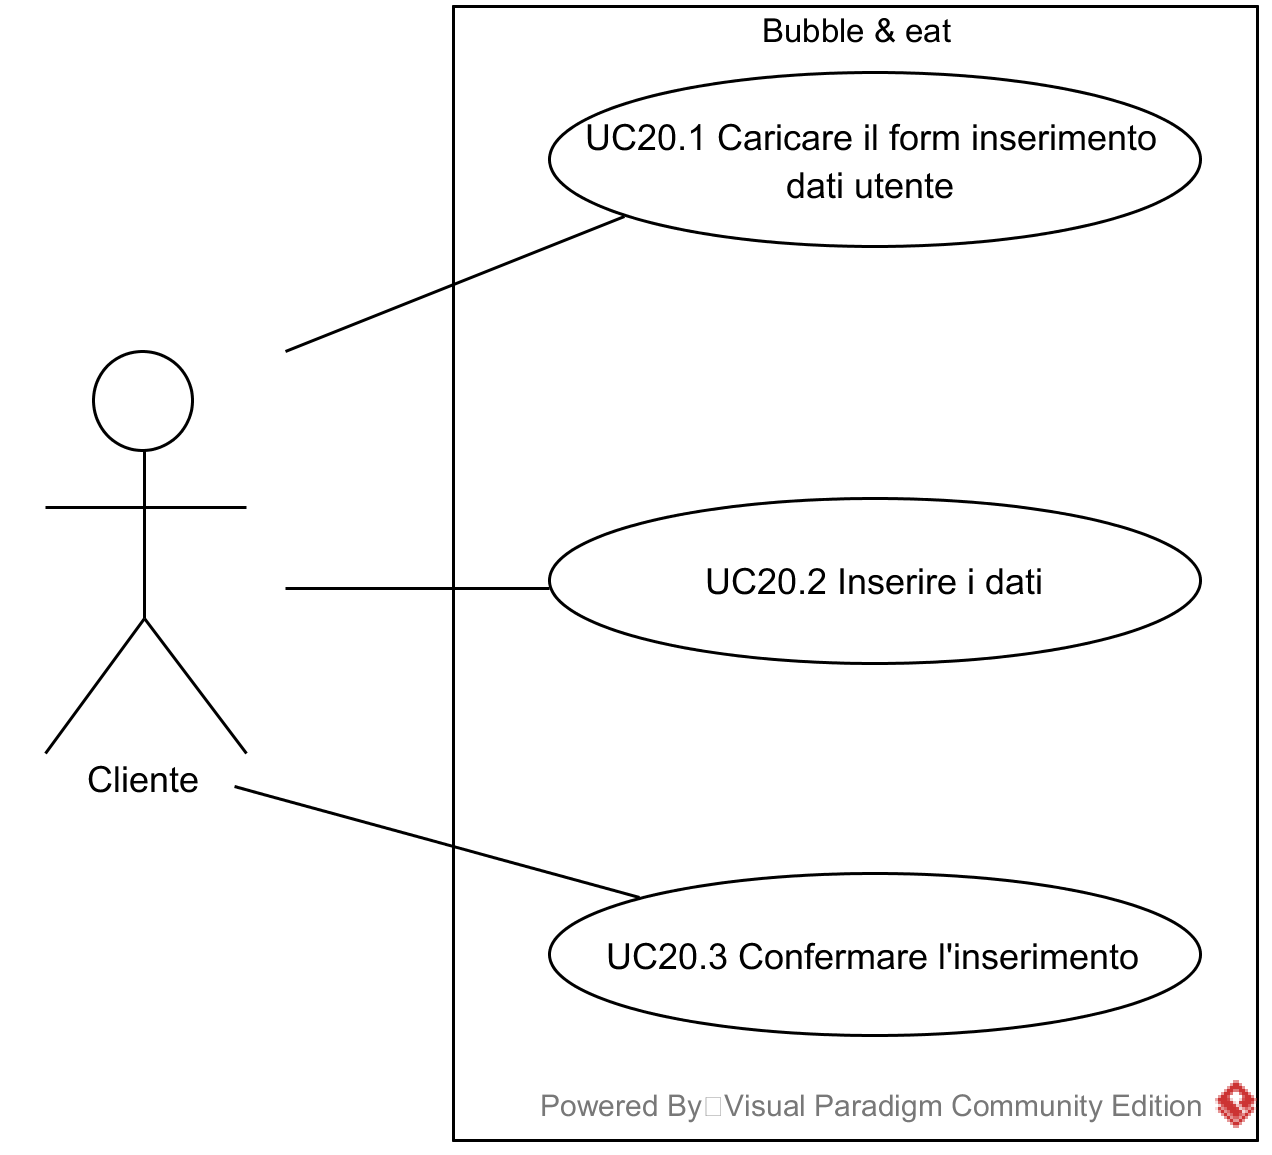
\includegraphics[width=15cm]{../../documenti/AnalisiDeiRequisiti/Diagrammi_img/usecase/uc3_1.png}
	\caption{\UCCaption{} Registrazione dei propri dati personali}
\end{figure}

%\begin{figure}[H]
%	\centering
%	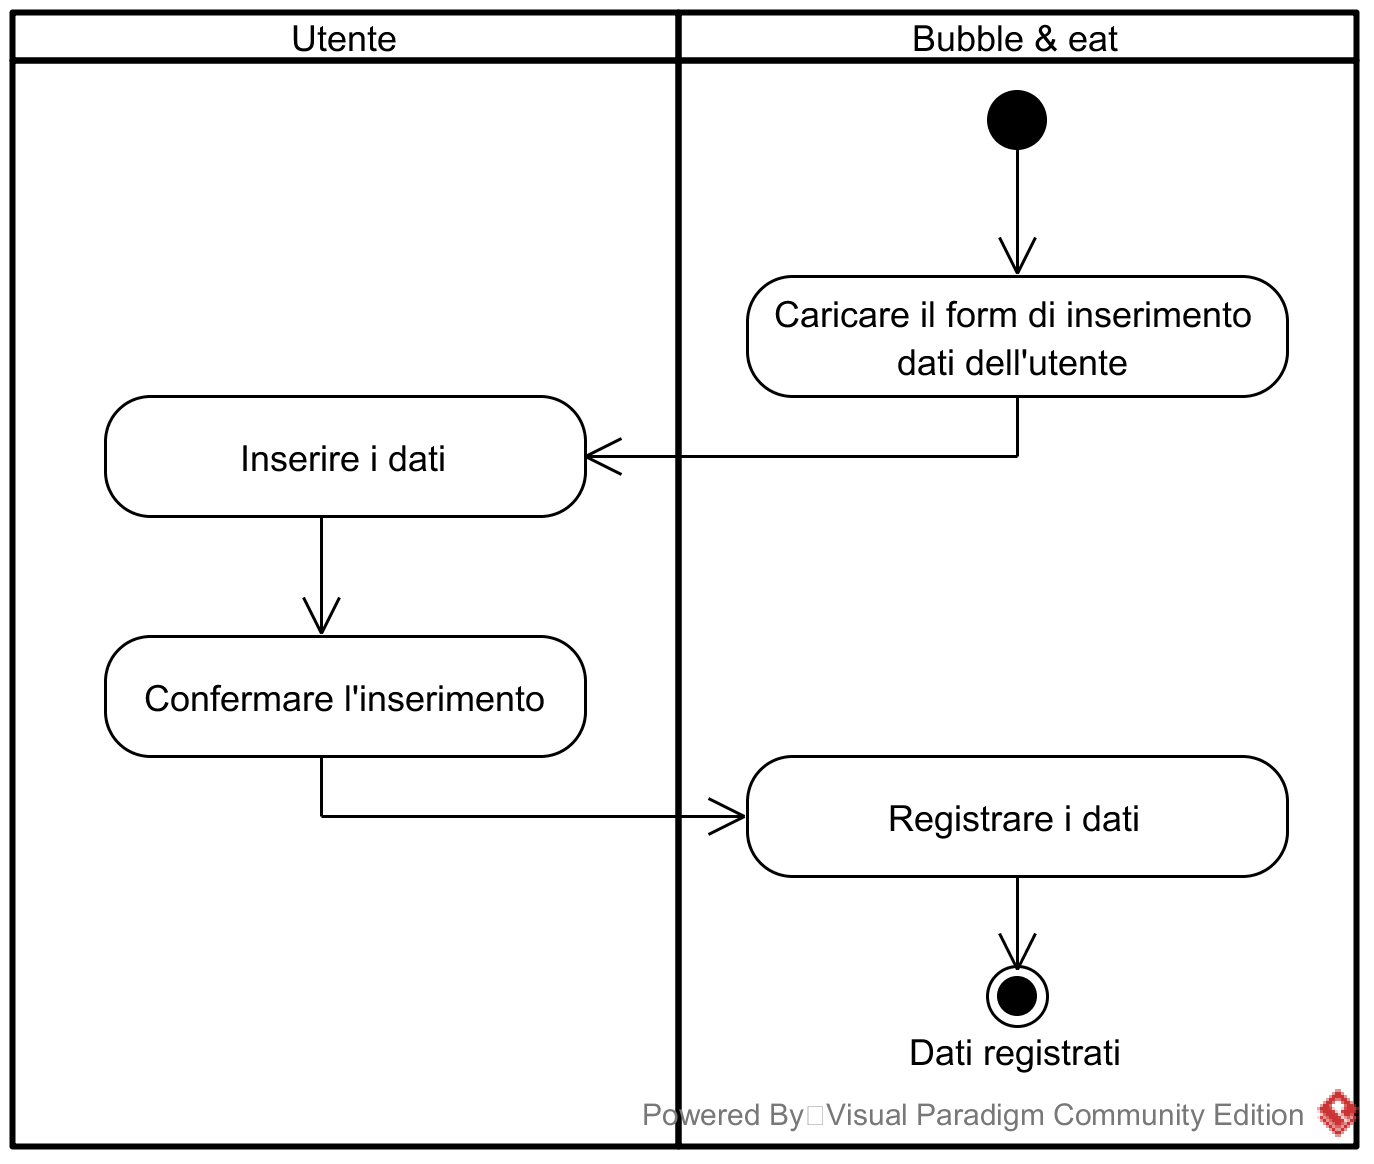
\includegraphics[height=10cm]{../../documenti/AnalisiDeiRequisiti/Diagrammi_img/attivita/uc_bubble_registrare_dati.png}
%	\caption{Diagramma di attività - Registrazione dei propri dati personali}
%\end{figure}

\begin{itemize}
	\item \textbf{Attori:}
	\\Cliente.
	\item \textbf{Scopo e descrizione:} 
	\\Registrare il proprio indirizzo e il proprio nome e cognome in modo tale da segnalarli all'azienda come destinazione per la spedizione del cibo.
	\item \textbf{Precondizioni:}
	\begin{itemize}
		\item Avere Rocket.Chat.
		\item Avere la bubble del ristorante selezionato.
	\end{itemize}
	\item \textbf{Flusso principale degli eventi:}
	\begin{itemize}
		\item Viene caricato il form di inserimento dati dell'utente \ref{UC3.1.1}.
		\item L'utente inserisce i dati \ref{UC3.1.2}.
		\item L'utente conferma l'inserimento \ref{UC3.1.3}.
	\end{itemize}
	\item \textbf{Post-condizione:}
	\\I dati dell'utente sono stati registrati nella bubble memory.
\end{itemize}

\UCF{Caricare form inserimento dati utente}{UC3.1.1}

\begin{itemize}
	\item \textbf{Attori:}
	\\Cliente.
	\item \textbf{Scopo e descrizione:} 
	\\Dare la possibilità di inserire i propri dati con lo scopo di segnalarli al locale per il corretto funzionamento del servizio.
	\item \textbf{Precondizioni:}
	\begin{itemize}
		\item Avere Rocket.Chat.
		\item Avere la bubble del ristorante selezionato.
	\end{itemize}
	\item \textbf{Flusso principale degli eventi:}
	\\Il form per l'inserimento dei dati utente viene caricato.
	\item \textbf{Post-condizione:}
	\\Nella bubble è presente il form per l'inserimento dei dati.
\end{itemize}

\UCF{Inserire i dati}{UC3.1.2}

\begin{itemize}
	\item \textbf{Attori:}
	\\Cliente.
	\item \textbf{Scopo e descrizione:} 
	\\Questo metodo permette all'utente di inserire il proprio indirizzo e il proprio nome e cognome con il fine di segnalarlo all'azienda, in modo tale da avere una destinazione per la spedizione del cibo.
	\item \textbf{Precondizioni:}
	\begin{itemize}
		\item Avere Rocket.Chat.
		\item Avere la bubble del ristorante selezionato.
	\end{itemize}
	\item \textbf{Flusso principale degli eventi:}
	\\L'utente seleziona i campi del form di inserimento e digita le informazioni.
	\item \textbf{Post-condizione:}
	\\I dati dell'utente sono stati inseriti.
\end{itemize}

\UCF{Conferma inserimento}{UC3.1.3}

\begin{itemize}
	\item \textbf{Attori:}
	\\Cliente.
	\item \textbf{Scopo e descrizione:} 
	\\Questo metodo permette all'utente di confermare l'inserimento dei dati inseriti nel form di registrazione.
	\item \textbf{Precondizioni:}
	\begin{itemize}
		\item Avere Rocket.Chat.
		\item Avere la bubble del ristorante selezionato.
	\end{itemize}
	\item \textbf{Flusso principale degli eventi:}
	\\Con l'apposito comando il Cliente conferma che i dati precedentemente immessi al caso d'uso \ref{UC3.1.2} siano corretti.
	\item \textbf{Post-condizione:}
	\\I dati confermati sono presenti nella memoria della bubble.
\end{itemize}

\UC{Guardare il menu}{UC3.2}

\begin{figure}[H]
	\centering
	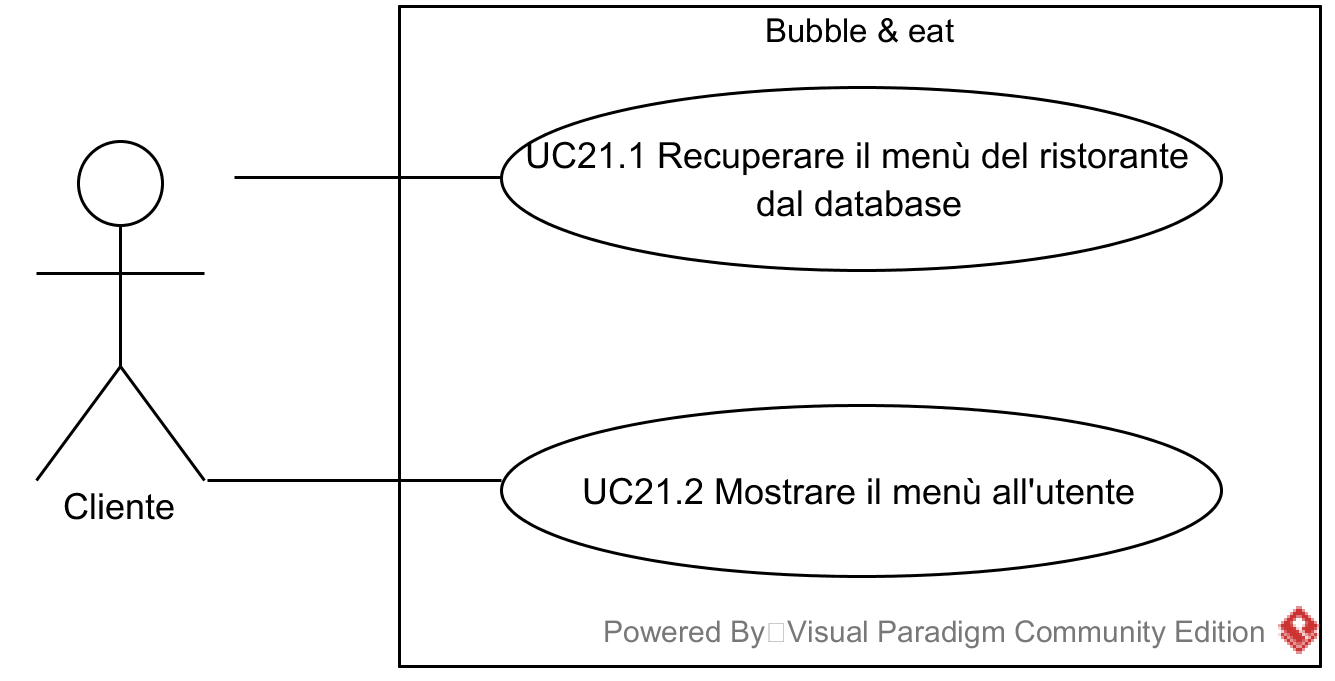
\includegraphics[width=15cm]{../../documenti/AnalisiDeiRequisiti/Diagrammi_img/usecase/uc3_2.png}
	\caption{\UCCaption{} Guardare il menu}
\end{figure}

%\begin{figure}[H]
%	\centering
%	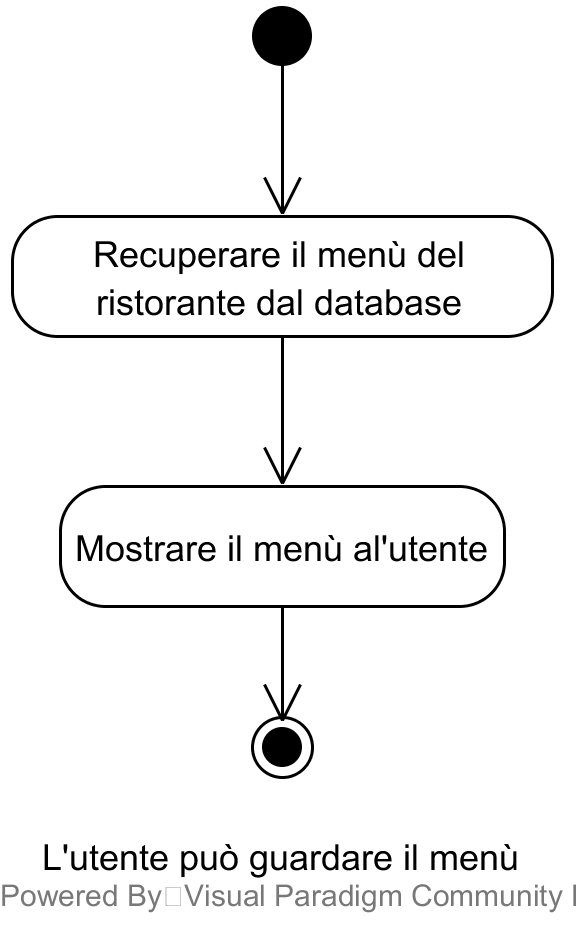
\includegraphics[height=10cm]{../../documenti/AnalisiDeiRequisiti/Diagrammi_img/attivita/uc_bubble_guardare_menu.png}
%	\caption{Diagramma di attività - Guardare il menu}
%\end{figure}

\begin{itemize}
	\item \textbf{Attori:}
	\\Cliente.
	\item \textbf{Scopo e descrizione:} 
	\\Il Cliente consulta il menu.
	\item \textbf{Precondizioni:}
	\begin{itemize}
		\item Avere Rocket.Chat.
		\item Avere la bubble del ristorante selezionato.
		\item Essere loggato nella bubble.
	\end{itemize}
	\item \textbf{Flusso principale degli eventi:}
	\begin{itemize}
		\item Viene recuperato il menu del ristorante dal database \ref{UC3.2.1}.
		\item Il menu caricato viene mostrato all'utente \ref{UC3.2.2}.
	\end{itemize}
	\item \textbf{Post-condizione:}
	\\Il menu è visualizzato sulla bubble.
\end{itemize}

\UCF{Recuperare il menu del ristorante dal database}{UC3.2.1}

\begin{itemize}
	\item \textbf{Attori:}
	\\Cliente.
	\item \textbf{Scopo e descrizione:} 
	\\Recuperare dal database le voci del menu del ristorante.
	\item \textbf{Precondizioni:}
	\begin{itemize}
		\item Avere Rocket.Chat.
		\item Avere la bubble del ristorante selezionato.
		\item Essere loggato nella bubble.
	\end{itemize}
	\item \textbf{Flusso principale degli eventi:}
	\\L'utente invia la richiesta di visualizzazione del menu e la bubble lo carica dal database.
	\item \textbf{Post-condizione:}
	\\Le informazioni sul menu sono state recuperate dalla bubble.
\end{itemize}

\UCF{Mostrare il menu all'utente}{UC3.2.2}

\begin{itemize}
	\item \textbf{Attori:}
	\\Cliente.
	\item \textbf{Scopo e descrizione:} 
	\\Visualizzare il menu nella bubble.
	\item \textbf{Precondizioni:}
	\begin{itemize}
		\item Avere Rocket.Chat.
		\item Avere la bubble del ristorante selezionato.
		\item Essere loggato nella bubble.
	\end{itemize}
	\item \textbf{Flusso principale degli eventi:}
	\\Il menu viene mostrato all'utente.
	\item \textbf{Post-condizione:}
	\\Il menu è visualizzato sulla bubble.
\end{itemize}

\UC{Fare le ordinazioni}{UC3.3}

\begin{figure}[H]
	\centering
	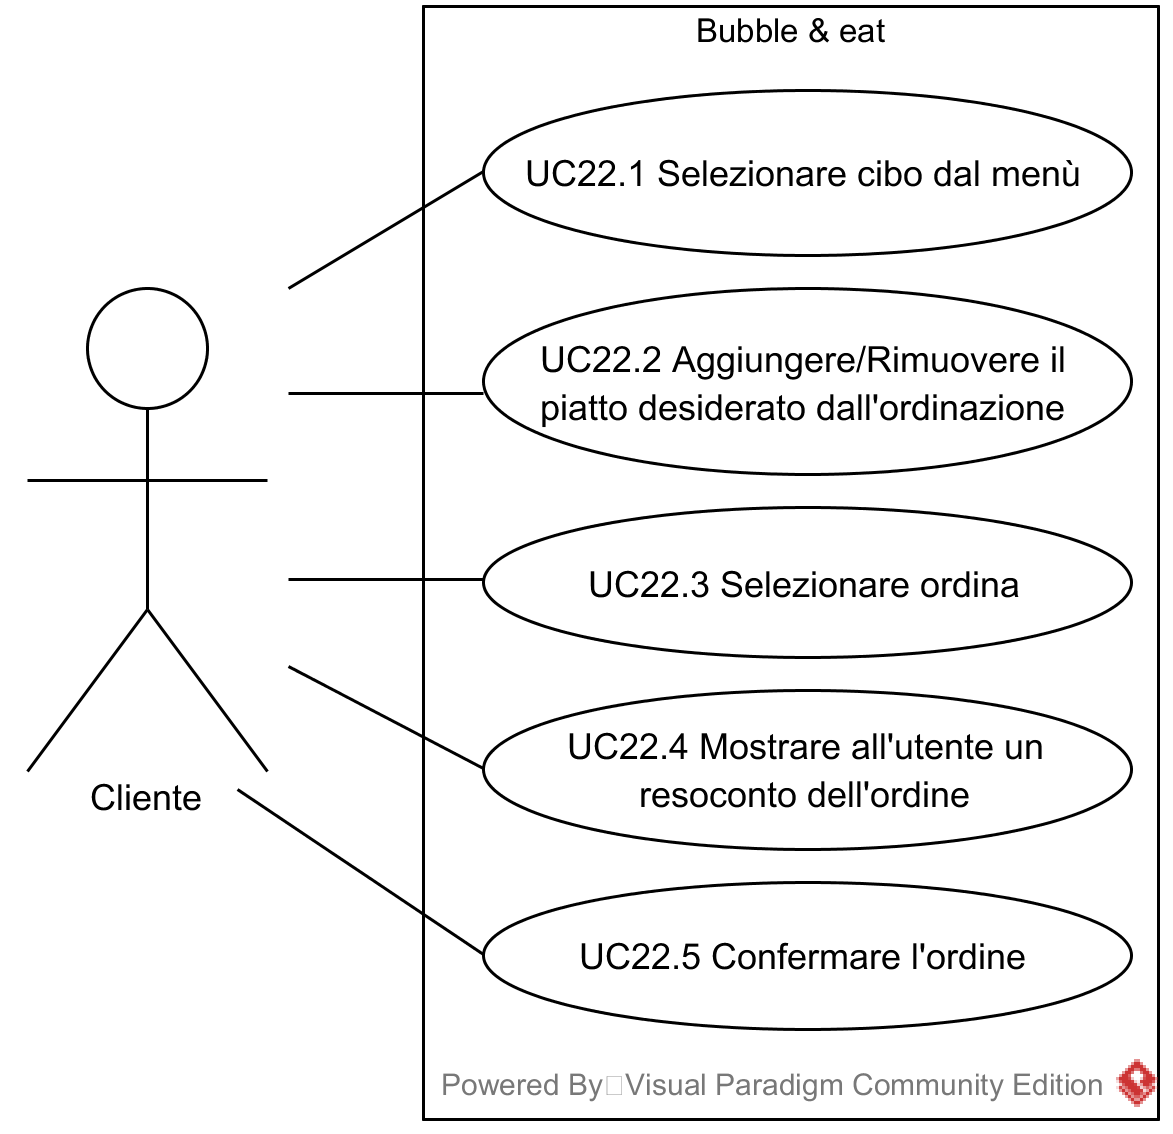
\includegraphics[width=15cm]{../../documenti/AnalisiDeiRequisiti/Diagrammi_img/usecase/uc3_3.png}
	\caption{\UCCaption{} Fare le ordinazioni}
\end{figure}

%\begin{figure}[H]
%	\centering
%	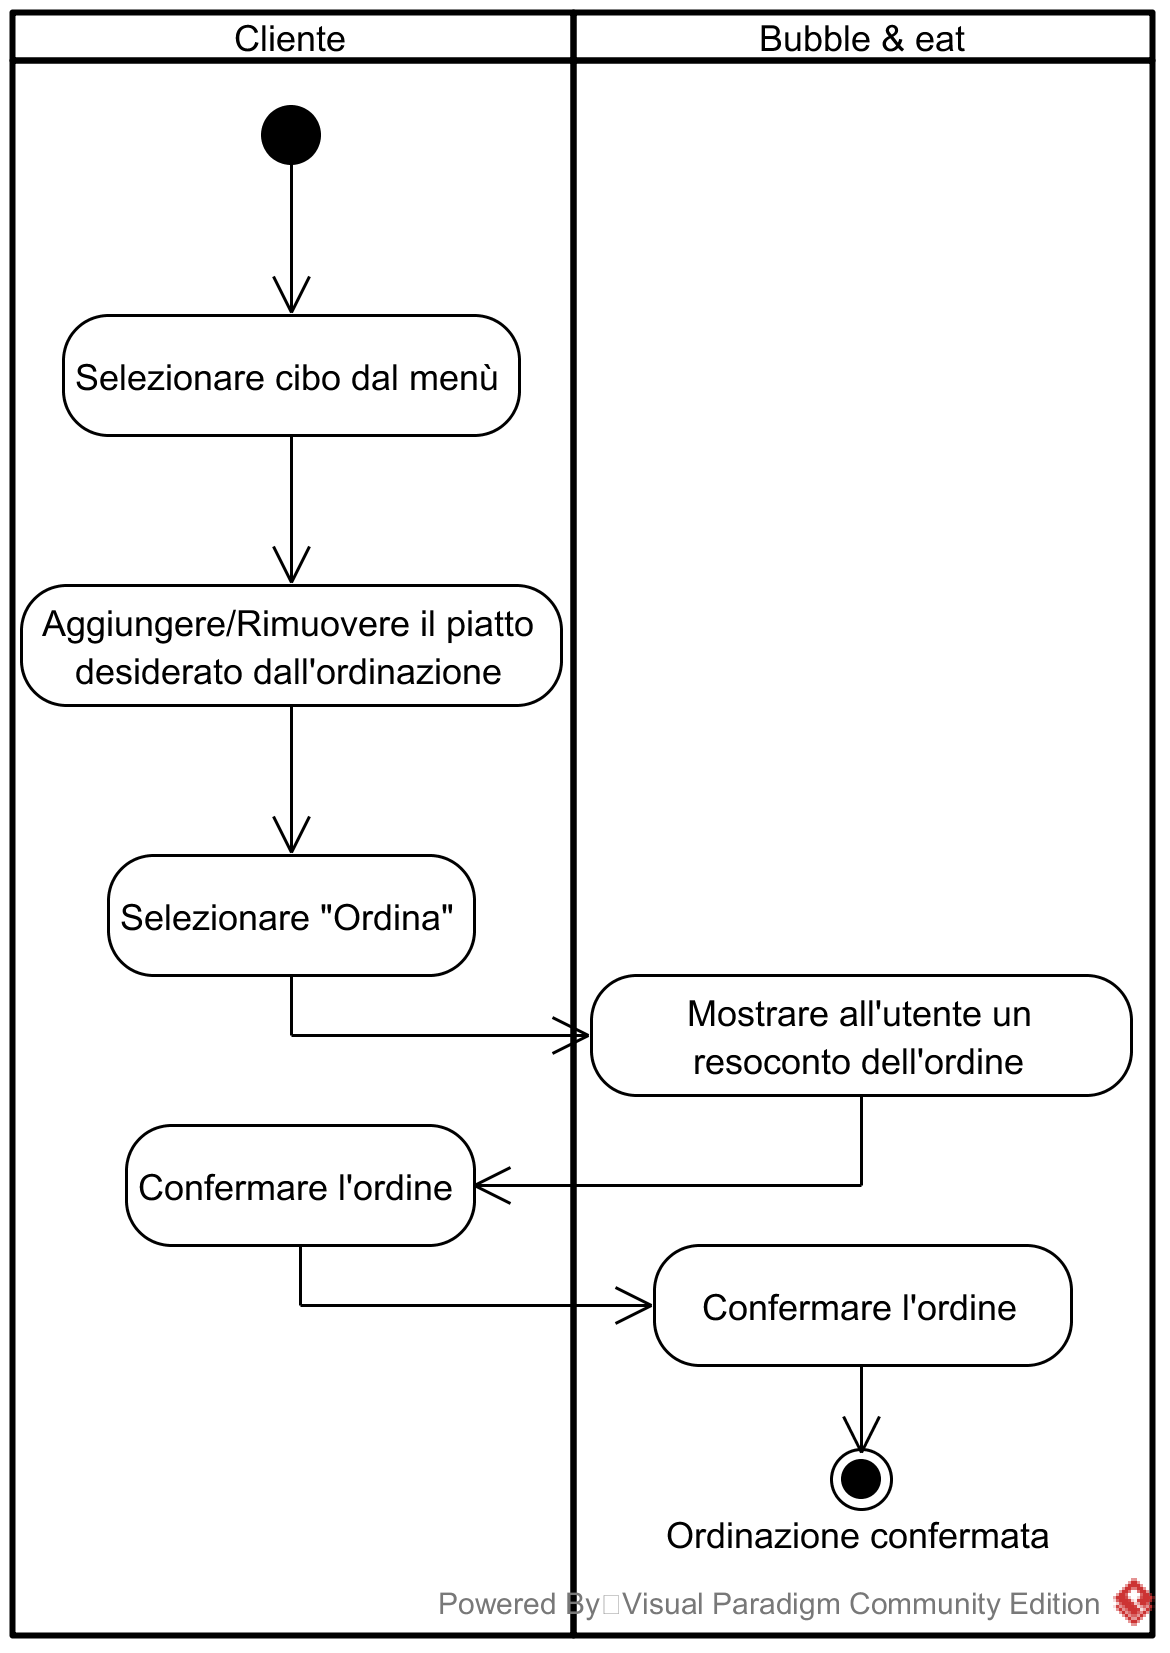
\includegraphics[height=10cm]{../../documenti/AnalisiDeiRequisiti/Diagrammi_img/attivita/uc_bubble_fare_ordinazioni.png}
%	\caption{Diagramma di attività - Fare le ordinazioni}
%\end{figure}

\begin{itemize}
	\item \textbf{Attori:}
	\\Cliente.
	\item \textbf{Scopo e descrizione:} 
	\\Selezionare i piatti e le quantità relative ad ogni pietanza.
	\item \textbf{Precondizioni:}
	\begin{itemize}
		\item Avere Rocket.Chat.
		\item Avere la bubble del ristorante selezionato.
		\item Essere loggato nella bubble.
	\end{itemize}
	\item \textbf{Flusso principale degli eventi:}
	\begin{itemize}
		\item Visualizzare menu \ref{UC3.2}.
		\item Selezionare cibi dal menu \ref{UC3.3.1}.
		\item Aggiungere/Rimuovere il cibo selezionato all'ordine \ref{UC3.3.2}.
		\item Selezionare \virgolette{Ordina} \ref{UC3.3.3}.
		\item Mostrare all'utente un resoconto dell'ordine \ref{UC3.3.4}.
		\item Confermare l'ordine \ref{UC3.3.5}.
	\end{itemize}
	\item \textbf{Post-condizione:}
	\\L'ordinazione viene aggiornata.
\end{itemize}

\UCF{Selezionare cibo dal menu}{UC3.3.1}

\begin{itemize}
	\item \textbf{Attori:}
	\\Cliente.
	\item \textbf{Scopo e descrizione:} 
	\\Selezionare voce di menu e relativa quantità.
	\item \textbf{Precondizioni:}
	\begin{itemize}
		\item Avere Rocket.Chat.
		\item Avere la bubble del ristorante selezionato.
		\item Essere loggato nella bubble.
		\item Aver caricato il menu del ristorante \ref{UC3.2}.
	\end{itemize}
	\item \textbf{Flusso principale degli eventi:}
	\begin{itemize}
		\item L'utente scorre la lista dei cibi ne seleziona voci e relative quantità.
	\end{itemize}
	\item \textbf{Post-condizione:}
	\\L'utente ha selezionato almeno un piatto dal menu.
\end{itemize}

\UCF{Aggiungere/Rimuovere il piatto desiderato dall'ordinazione}{UC3.3.2}

\begin{itemize}
	\item \textbf{Attori:}
	\\Cliente.
	\item \textbf{Scopo e descrizione:} 
	\\Aggiungere oppure rimuovere alla propria ordinazione un'unità del piatto selezionato.
	\item \textbf{Precondizioni:}
	\begin{itemize}
		\item Avere Rocket.Chat.
		\item Avere la bubble del ristorante selezionato.
		\item Essere loggato nella bubble.
	\end{itemize}
	\item \textbf{Flusso principale degli eventi:}
	\\L'utente invoca l'apposito comando sulla bubble per poter rimuovere o aggiungere il piatto selezionato al proprio ordine.
	\item \textbf{Post-condizione:}
	\\L'ordinazione viene aggiornata correttamente con il piatto selezionato.
\end{itemize}

\UCF{Selezionare \virgolette{Ordina}}{UC3.3.3}

\begin{itemize}
	\item \textbf{Attori:}
	\\Cliente.
	\item \textbf{Scopo e descrizione:} 
	\\Il Cliente effettua l'ordine selezionando l'apposita funzione.
	\item \textbf{Precondizioni:}
	\begin{itemize}
		\item Avere Rocket.Chat.
		\item Avere la bubble del ristorante selezionato.
		\item Essere loggato nella bubble;
		\item Aver selezionato cibi e quantità dal menu \ref{UC3.3.1} \ref{UC3.3.2}.
	\end{itemize}
	\item \textbf{Flusso principale degli eventi:}
	\\L'utente invoca l'apposito comando di ordine sulla bubble.
	\item \textbf{Post-condizione:}
	\\L'ordinazione è registrata ed è in attesa di conferma.
\end{itemize}

\UCF{Mostrare all'utente un resoconto dell'ordine}{UC3.3.4}

\begin{itemize}
	\item \textbf{Attori:}
	\\Cliente.
	\item \textbf{Scopo e descrizione:} 
	\\Mostrare all'utente un resoconto dell'ordine che sta per effettuare prima della conferma.
	\item \textbf{Precondizioni:}
	\begin{itemize}
		\item Avere Rocket.Chat.
		\item Avere la bubble del ristorante selezionato.
		\item Essere loggato nella bubble.
		\item Aver selezionato cibi e quantità dal menu \ref{UC3.3.1} \ref{UC3.3.2}.
	\end{itemize}
	\item \textbf{Flusso principale degli eventi:}
	\\L'utente seleziona \virgolette{Mostra resoconto} e riceve dunque una lista completa di tutto e solo quello che sta per ordinare, insieme al prezzo totale dell'ordine.
	\item \textbf{Post-condizione:}
	\\L'utente visualizza un resoconto dell'ordine prima di confermarlo.
\end{itemize}

\UCF{Confermare l'ordine}{UC3.3.5}

\begin{itemize}
	\item \textbf{Attori:}
	\\Cliente.
	\item \textbf{Scopo e descrizione:} 
	\\Confermare che quanto mostrato nel caso d'uso \ref{UC3.3.4} è corretto e salvare l'ordinazione nella memoria della bubble.
	\item \textbf{Precondizioni:}
	\begin{itemize}
		\item Avere Rocket.Chat.
		\item Avere la bubble del ristorante selezionato.
		\item Essere loggato nella bubble.
		\item Aver effettuato l'ordinazione \ref{UC3.3.4}.
	\end{itemize}
	\item \textbf{Flusso principale degli eventi:}
	\\L'utente invoca l'apposito comando sulla bubble.
	\item \textbf{Post-condizione:}
	\\L'ordinazione viene salvata nella memoria della bubble.
\end{itemize}

\UC{Inviare l'ordinazione}{UC3.4}

\begin{figure}[H]
	\centering
	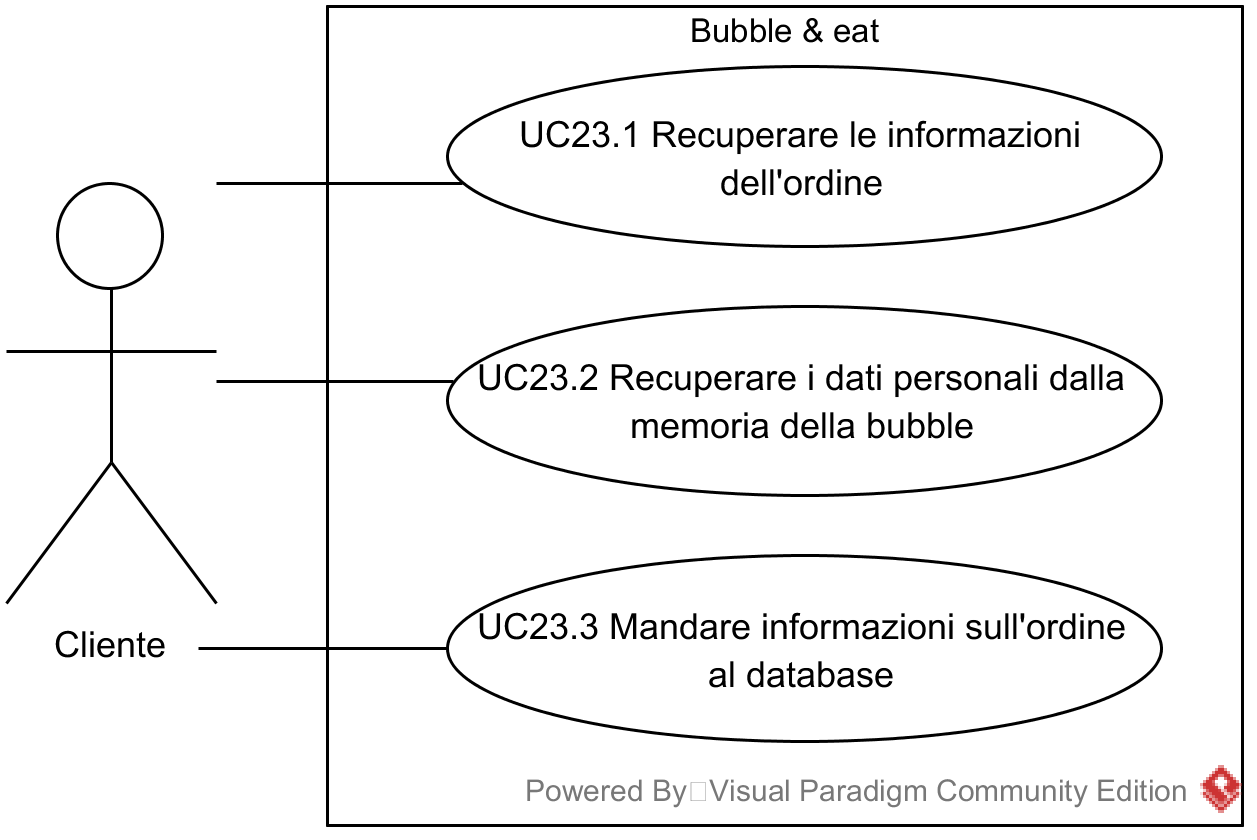
\includegraphics[width=15cm]{../../documenti/AnalisiDeiRequisiti/Diagrammi_img/usecase/uc3_4.png}
	\caption{\UCCaption{} Inviare l'ordinazione}
\end{figure}

%\begin{figure}[H]
%	\centering
%	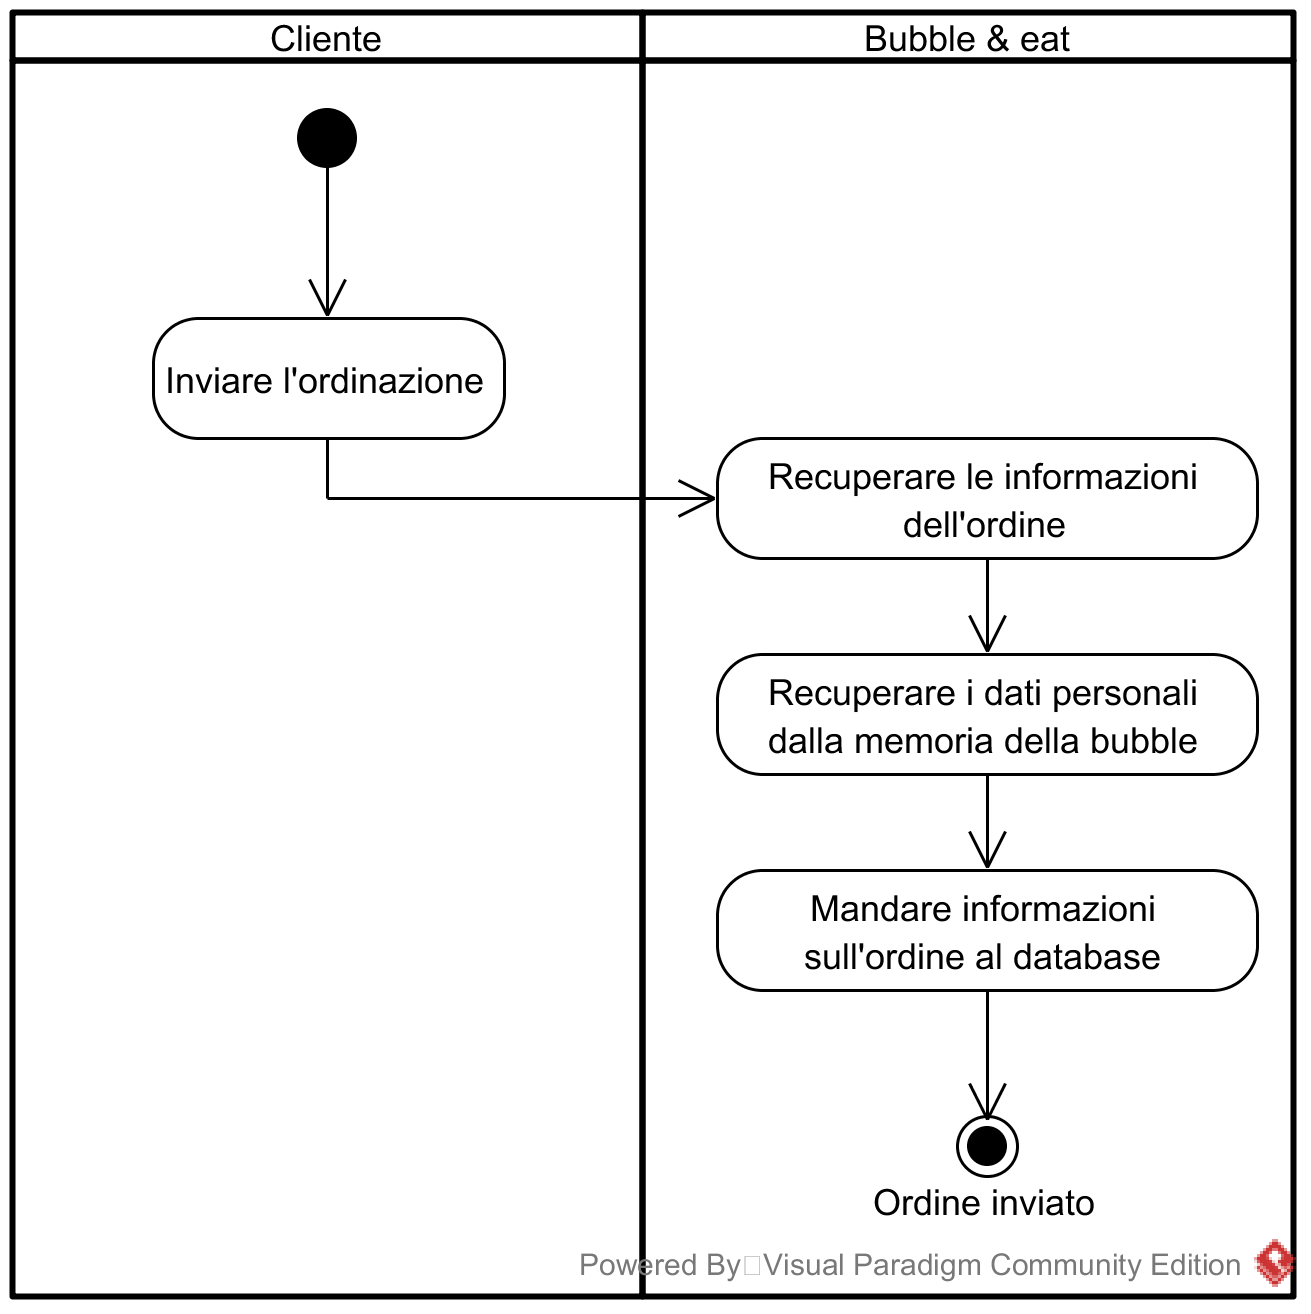
\includegraphics[height=10cm]{../../documenti/AnalisiDeiRequisiti/Diagrammi_img/attivita/uc_bubble_inviare_ordinazione.png}
%	\caption{Diagramma di attività - Inviare l'ordinazione}
%\end{figure}

\begin{itemize}
	\item \textbf{Attori:}
	\\Cliente.
	\item \textbf{Scopo e descrizione:} 
	\\Selezionare il comando di invio dell'ordinazione.
	\item \textbf{Precondizioni:}
	\begin{itemize}
		\item Avere Rocket.Chat.
		\item Avere la bubble del ristorante selezionato.
		\item Essere loggato nella bubble.
		\item Avere un'ordinazione non vuota.
	\end{itemize}
	\item \textbf{Flusso principale degli eventi:}
	\begin{itemize}
		\item Vengono recuperate dalla memoria della bubble le informazioni sull'ordine \ref{UC3.4.1}.
		\item Vengono recuperate le informazioni sui dati personali del Cliente dalla memoria della bubble \ref{UC3.4.2}.
		\item Vengono inviate le informazioni sull'ordine al database \ref{UC3.4.3}.
	\end{itemize}
	\item \textbf{Post-condizione:}
	\\L'ordinazione viene inviata.
\end{itemize}

\UCF{Recuperare le informazioni dell'ordine}{UC3.4.1}

\begin{itemize}
	\item \textbf{Attori:}
	\\Cliente.
	\item \textbf{Scopo e descrizione:} 
	\\Prelevare dalla memoria della bubble i dati relativi all'ordinazione confermata nell'\ref{UC3.3.5}.
	\item \textbf{Precondizioni:}
	\begin{itemize}
		\item \ref{UC3.3.5}.
		\item Avere Rocket.Chat.
		\item Avere la bubble del ristorante selezionato.
		\item Essere loggato nella bubble.
	\end{itemize}
	\item \textbf{Flusso principale degli eventi:}
	\\L'utente invoca con l'apposito comando l'\ref{UC3.4}.
	\item \textbf{Post-condizione:}
	\\I dati desiderati, relativi all'ordinazione effettuata nell'\ref{UC3.3}, sono stati recuperati. 
\end{itemize}

\UCF{Recuperare informazioni dei dati personali dalla memoria della bubble}{UC3.4.2}

\begin{itemize}
	\item \textbf{Attori:}
	\\Cliente.
	\item \textbf{Scopo e descrizione:} 
	\\Ottenere informazioni riguardanti il Cliente dalla memoria della bubble.
	\item \textbf{Precondizioni:}
	\begin{itemize}
		\item Avere Rocket.Chat.
		\item Avere la bubble del ristorante selezionato.
		\item Essere loggato nella bubble.
		\item Avere un'ordinazione da inviare non vuota.
	\end{itemize}
	\item \textbf{Flusso principale degli eventi:}
	\\Vengono recuperate le informazioni sui dati personali del Cliente dalla memoria della bubble.
	\item \textbf{Post-condizione:}
	\\I dati personali del Cliente sono stati letti dalla memoria della bubble.
\end{itemize}

\UCF{Mandare informazioni sull'ordine al database}{UC3.4.3}

\begin{itemize}
	\item \textbf{Attori:}
	\\Cliente.
	\item \textbf{Scopo e descrizione:} 
	\\Invio delle informazioni al database.
	\item \textbf{Precondizioni:}
	\begin{itemize}
		\item Avere Rocket.Chat.
		\item Avere la bubble del ristorante selezionato.
		\item Essere loggato nella bubble.
		\item Avere un'ordinazione non vuota.
	\end{itemize}
	\item \textbf{Flusso principale degli eventi:}
	\\Le informazioni sull'ordinazione vengono mandate al database.
	\item \textbf{Post-condizione:}
	\\L'ordinazione è salvata nel database.
\end{itemize}